\chapter{Algoritmi di inferenza per reti Bayesiane}
In questo capitolo verranno trattati gli aspetti legati all'implementazione degli algoritmi di MPE e MAP, verranno analizzati i punti chiave dell’implementazione, partendo da aspetti di più basso livello (come la struttura dati scelta per rappresentare la cpt) a quelli di più alto livello (come la descrizione degli algoritmi stessi di MAP ed MPE).

\section{Implementazione}
L’implementazione è stata realizzata in python partendo completamente da zero, ovvero si è scelto di non usufruire della possibilità di avvalersi del codice fornito dalla repository ufficiale \texttt{aimacode}. Questa scelta ha portato ad un sostanzioso incremento del lavoro da svolgere coadiuvato però da una maggiore libertà espressiva e da una maggior consapevolezza delle operazioni effettuate.

\subsection{CPT}
La cpt richiede una struttura dati non banale per poter essere rappresentata. Tale elemento è formato da una lista di variabili associate, una lista di assegnamenti (la cui quantità dipende dai domini delle variabili associate) e un valore in corrispondenza ad ogni assegnamento. Sono stati provati diversi approcci per la rappresentazione di questi oggetti, cercando di trovare un equilibrio tra efficienza e comodità di accesso ai dati. Dopo alcune idee scartate (come liste di dizionari o matrici) si è optato per una lista di oggetti (Assignment) ognuno aventi come parametri: variabili, assignment e rispettivo valore. Questo metodo si è rivelato particolarmente comodo in quanto permette di avere sempre a disposizione tutte le informazioni necessarie e di poterle gestire in modo dinamico, al prezzo di una ridondanza del nome delle variabili associate, che viene ripetuto per ogni riga della cpt. Quando si è passati a lavorare su reti più grandi si è però subito palesato il limite di questo sistema di rappresentazione, ovvero l’ efficienza. Facendo un’analisi dei tempi di calcolo ci si è accorti infatti che la maggior parte del tempo veniva trascorsa nella routine di sum out.

\subsection{Implementazione del'operazione di  Sum Out}

\begin{minipage}{\linewidth}
	\centering
	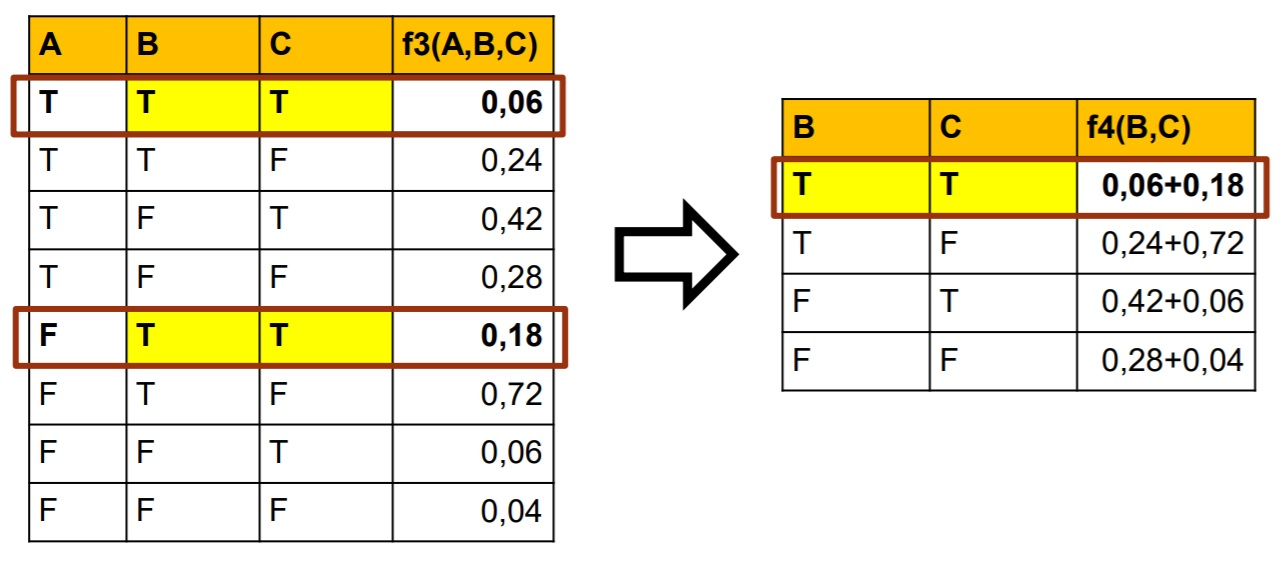
\includegraphics[width=0.9\linewidth]{map_teoria}
	\captionof{figure}{Esempio grafico del processo di Sum Out preso dalle slide a lezione.} 
	\label{map_teoria} 
\end{minipage}

Andiamo ora ad analizzare nel dettaglio questa procedura e ad individuare l’istruzione da ottimizzare per evitare il collo di bottiglia nel processore. L’operazione di sum-out consiste nella trasformazione di una cpt verso una seconda, il cui numero di colonne viene ridotto (e quindi anche di righe). Togliendo una colonna, molti degli assegnamenti che si differenziavano soltanto per il valore di tale colonna ora coincideranno (il numero di questi assegnamenti dipende dalla cardinalità del dominio della variabili eliminata). Di tutti gli assegnamenti ripetuti solo uno verrà assegnato alla nuova cpt e come valore associato a quell' assegnamento si utilizzarà la somma di tutti i valori associati agli assegnamenti ripetuti. Inizialmente questa operazione veniva eseguita ciclando su tutte le righe della cpt, per ogni riga si eliminava l’ assegnamento corrispondente a quello della variabile target e il risultato ottenuto lo si inseriva nella nuova cpt. Prima dell’inserimento però si doveva verificare che questo assegnamento non fosse già stato inserito in qualche passo precedente (questa operazione richiede di ispezionare tutta la nuova cpt). In base a questa verifica si decideva se creare una nuova riga con rispettivo valore o se limitarsi a sommare il nuovo valore con quello già inserito precedentemente in quella riga. Sebbene rimanga inevitabile ciclare per tutte le righe della cpt originaria, la medesima operazione non è necessaria per la cpt derivata. Ciò che effettivamente viene svolto  è una ricerca mediante una chiave, che può essere realizzata in tempo logaritmico se si usa una struttura a dizionario. Per cui si è scelto di modificare la struttura dati in un Oggetto avente come attributi una la lista (su cui sono segnate le variabili di associate a quella cpt, in modo da averle sempre disponibili ma senza ridondanze) e un dizionario del tipo: \texttt{cpt[tuple(assignment)] = value} (ovvero un dizionario in cui la chiave è data dagli assegnamenti delle variabili e il valore è dato  dalla cifra associata ad ogni assegnamento). Questo cambiamento ha snellito ulteriormente il codice permettendo di eliminare diverse funzioni ausiliarie e ha migliorato di molto i tempi di calcolo. A titolo esemplificativo lasciamo qui di seguito un estratto del codice sorgente dell’ operazione di sum out.

\begin{minipage}{\linewidth}
	\centering
	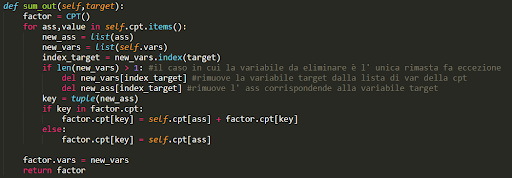
\includegraphics[width=0.9\linewidth]{codice}
	\captionof{figure}{Sorgente del metodo di Sum Out.} 
	\label{codice} 
\end{minipage}
 

\subsection{Altri metodi della classe CPT}
Gli altri metodi rilevanti della classe CPT sono:

\begin{itemize}
\item \textbf{Max Out}\\ 
Questo metodo è molto simile a quello di sum out se non per il valore associato agli assegnamenti che non è più calcolato mediante la somma dei due fattori ma che corrisponde al maggiore dei due.

\item \textbf{Pointwise Product}\\ 
Questo metodo combina due cpt andandone a creare una terza le cui variabili sono date dall’unione insiemistica delle variabili associate alle cpt di input. Per quanto riguarda il valore dei nuovi assignment prodotti, questo è dato dalla moltiplicazione dei dei valori degli assignemnt che sono stati combinati.

\item \textbf{Miglior assegnamento}\\
Questo metodo viene utilizzato nella retropropagazione degli assignment (che verrà spiegato più avanti nel paragrafo \ref{retropropagazione}). Data una lista di variabili (sottoinsieme di tutte le variabili della cpt) ed i rispettivi valori di assignment, restituisce il valore massimo tra tutti quelli associati agli assignments che combaciano con l'input ricevuto.
\end{itemize}
 
\subsection{Parser}
Avendo realizzato il software in python, non è stato possibile utilizzare il parser java fornito su moodle quindi si è deciso di svilupparne uno nostro adattandolo alle classi del nostro progetto. Durante parsificazione del file viene anche creato il grafo da cui estrarre l’ordine topologico, necessario poi per lo sviluppo degli algoritmi di MAP ed MPE.

\subsection{Grafo}
Questa classe costruisce il grafo che viene utilizzato per individuare l’ordine topologico dei nodi sulla rete. Tale struttura viene costruita e utilizzata solo durante la parsificazione del file e non influisce sui tempi di esecuzione dell’ algoritmo generale.
Ogni volta che si parsifica un nodo si trovano informazioni sui genitori di tale nodo. Nel dizionario rappresentante il grafo generale, invece di associare ogni nodo ai genitori, associamo ogni genitore ai rispettivi figli. In questo modo è possibile individuare facilmente quando un certo nodo è una foglia semplicemente verificando che non sia presente nel grafo (non è mai apparso tra i parent di qualche nodo). Per quanto riguarda i nodi root, questa caratteristica è facilmente inferibile dal file stesso. A questo punto abbiamo una lista di root da porre ad inizio dell’ ordine topologico e una lista di foglia da aggiungere in coda, restano da riordinare i nodi centrali. Dal momento che le reti bayesiani sono dei grafi e non degli alberi, sono possibili alcuni casi non banali da gestire, come ad esempio un collegamento diretto tra un nodo genitore, un nodo figlio e tra lo stesso nodo genitore ed il nodo figlio del suo nodo figlio. Questo tipo di problematiche ha reso impraticabili alcune implementazioni particolarmente vantaggiose dal punto di vista della complessità ma che non funzionavano su tutte le reti. L’algoritmo finale (che opera solo sulla lista non ordinata di nodi, da cui sono stati esclusi i nodi di root e quelli foglia) sposta i nodi nella lista ordinata solo se tutti i rispettivi parent sono già stati spostati, altrimenti passa ad analizzare il nodo successivo. Al termine della lista la ripercorre di nuovo da capo fino a che non sarà stato rimosso anche l’ultimo nodo. Nonostante scorra più volte la stessa lista non sono stati riscontrati particolari attese durante il parsing e il controllo sulla presenza dei parent assicura che il nodo verrà sempre inserito dopo di essi.

\subsection{Menu}
Si è deciso di gestire l’interazione con l’utente mediante un menu per agevolare la possibilità di settare comodamente più variabili senza dover ricompilare e per poter scegliere a tempo di esecuzione che tipo di operazione eseguire (es: map, mpe o benchmark).


\begin{minipage}{\linewidth}
	\centering
	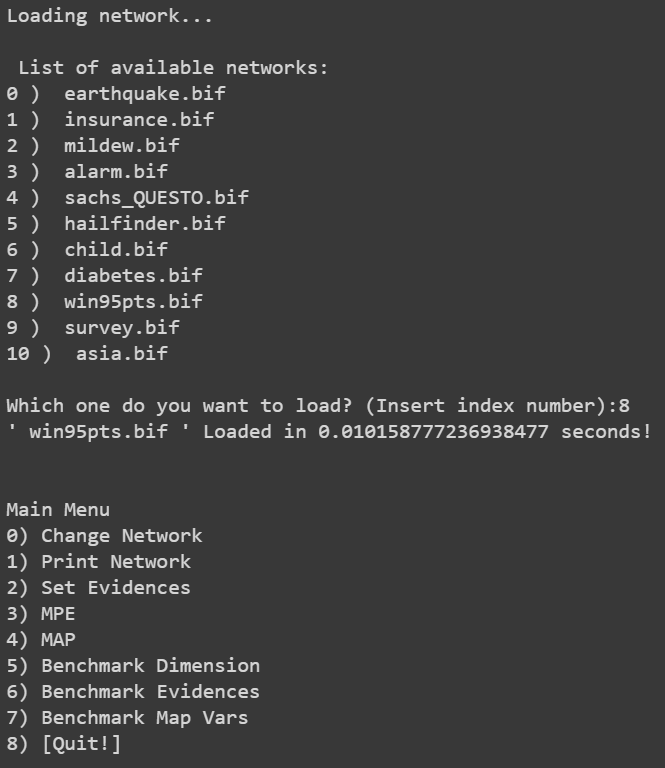
\includegraphics[width=0.5\linewidth]{menu}
	\captionof{figure}{Esempio di interazione con l' utente (si notino i tempi di attesa per il caricamente di win95pts, una rete di tipo "large").} 
	\label{codice} 
\end{minipage}

\section{Spiegazione MPE}
L’algoritmo di MPE segue un’impostazione molto vicina a quella proposta da Aimacode nel suo algoritmo di variable elimination. 
Sebbene siano state sperimentate più soluzioni per la gestione dei fattori prodotti durante l’esecuzione, alla fine si è optato per raccoglierli in una lista. Nel primo ciclo si percorre tutta la rete seguendo l’ordine topologico inverso e per ogni nodo se ne raccoglie la rispettiva cpt aggiungendola ad una lista. Durante questa operazione vengono rimosse tutte le entry contenenti assegnamenti in contraddizione con le evidenze fornite (se ce ne sono). Una volta aggiunto l’elemento si esegue un pointwise di tutti gli elementi attualmente presenti in lista che contengono la variabile associata al nodo target, e poi si esegue il max out sulla cpt risultate per eliminare tale variabile. Si prosegue quindi con una nuova lista avente il risultato appena ottenuto come unico elemento. Una volta completata la visita della rete si moltiplicano tutti gli elementi rimanenti nella lista e si calcola il valore massimo ottenuto in questa cpt finale. Questo valore verrà utilizzato per individuare il miglior assegnamento per tutti i nodi della rete. ( Spiegheremo in dettaglio questo metodo nel paragrafo \ref{retropropagazione}).

\section{Spiegazione MAP}
A differenza di MPE l’algoritmo richiede due cicli. Il primo ciclo è simile a quello visto in mpe ma oltre alla variabili di evidenza vengono ignorate anche quelle scelte come Map Var. Inoltre l’eliminazione dei fattori questa volta avviene con operazioni di sum out e non più max out. Il secondo ciclo avviene solo sulle restanti variabili map e consiste nella loro eliminazione tramite max out. Anche in questo caso si moltiplicano tutti i valori restanti nella lista per calcolare il valore totale da restituire e che verrà usato anche poi per il calcolo dei migliori assegnamenti dei nodi della rete.

\section{Retropropagazione dei migliori assegnamenti.}
Una volta individuato il valore finale (e quindi individuato il miglior assegnamento per l’ultimo nodo visitato) sarà possibile ripercorrere a ritroso la rete andando ad individuare i migliori assegnamenti per ogni nodo della rete. Per individuare tali valori si forniscono gli assegnamenti delle variabili padri (individuati dalla cpt dell’iterazione precedente) e si fissano tali valori facendo variare solo quello della variabile relativa al nodo, a quel punto si prende il valore massimo tra quelli disponibili. Si lascia qui di seguito un esempio per rendere più chiaro il procedimento.


\subsection{Esempio di Retropropagazione}\label{retropropagazione}
A titolo di esempio prendiamo la configurazione dell’esempio pubblicato su moodle. In quel caso otteniamo come valore risultante:

\lstset{language=Octave,basicstyle=\ttfamily}
\begin{lstlisting}[frame=single]
Rete Earthquake
Map Var: E,B,J,M
Best assignments
[0.9115897329]
\end{lstlisting}

Andando a esplorare in ordine topografico la rete, troviamo la cpt del primo noto (ovvero Burglary) con i valori aggiornati e troviamo facilmente la riga con l’assegnazione corretta

\lstset{language=Octave,basicstyle=\ttfamily}
\begin{lstlisting}[frame=single]
Current Node:  Burglary
Print CPT
['Burglary']
('True',)  ->  0.005803854
('False',)  ->  0.9115897329 -> max assignment
\end{lstlisting}

A questo punto passiamo all’iterazione successiva, tenendoci salvato il valore di (Burglary = False). Il nodo successivo è Earthquake.

\lstset{language=Octave,basicstyle=\ttfamily}
\begin{lstlisting}[frame=single]
Current Node:  Earthquake
Print CPT: 
['Earthquake', 'Burglary']
('True', 'True')  ->  0.0119705
('True', 'False')  ->  0.0135291 
('False', 'True')  ->  0.5803853999999999
('False', 'False')  ->  0.92079771 
\end{lstlisting}

A questo punto si procede isolando le righe in cui (Burglary = False) :

\lstset{language=Octave,basicstyle=\ttfamily}
\begin{lstlisting}[frame=single]
Current Node:  Earthquake
Print CPT: 
['Earthquake', 'Burglary']
('True', 'True')  ->  0.0119705
('True', 'False')  ->  0.0135291 -> candidate 
('False', 'True')  ->  0.5803853999999999
('False', 'False')  ->  0.92079771 -> candidate 
\end{lstlisting}

e se ne individua quella con valore massimo (0.92079771). Si aggiunga l’assegnamento di [Earthquake = False] alla lista e si proceda con le iterazioni successive. Andando ancora avanti si arriverà al nodo MaryCalls. Intuitivamente ci aspetteremmo di trovare Alarm ma essendo questa una variabili Non Map è stata eliminata dalla rete e i suoi figli sono diventati figli dei suoi parent. In sostanza il nodo MaryCalls ha come parent i parent di Alarm.

\lstset{language=Octave,basicstyle=\ttfamily}
\begin{lstlisting}[frame=single]
Current Node:  MaryCalls
Print CPT
['MaryCalls', 'Burglary', 'Earthquake']
('True', 'True', 'True')  ->  0.598525
('True', 'False', 'True')  ->  0.183055
('True', 'True', 'False')  ->  0.5922299999999999
('True', 'False', 'False')  ->  0.0095605 -> candidate 
('False', 'True', 'True')  ->  0.258975
('False', 'False', 'True')  ->  0.676455
('False', 'True', 'False')  ->  0.25677
('False', 'False', 'False')  ->  0.9395895 -> candidate 
\end{lstlisting}

Le informazioni su Burglary ed Earthquake sono esattamente quelle che abbiamo raccolto nelle iterazioni precedenti quindi possiamo continuare a reiterare il processo fino alla fine della visita arrivando alla conclusione:

\lstset{language=Octave,basicstyle=\ttfamily}
\begin{lstlisting}[frame=single]
Best assignments
[0.9115897329]

Burglary  ->  False
Earthquake  ->  False
MaryCalls  ->  False
JohnCalls  ->  False
\end{lstlisting}

\section{Verifica di correttezza delle implementazioni di MAP e MPE}
Una volta implementati gli algoritmi sono stati sperimentalmente verificati attraverso moltissime prove su varie configurazioni e su reti di diverse dimensioni. I risultati ottenuti sono stati confrontati con quelli forniti dall’ applicativo Samiam.






\section{Analisi delle performance}

Segue ora l’analisi dei risultati volta ad evidenziare le differenze principali tra il task di MPE e quello di MAP. Tale analisi verrà divisa in 4 punti, in ognuno dei quali si andrà ad analizzare un parametro diverso. 

\section{Reti Utilizzate}
I grafici sono stati ottenuti eseguendo i benchmark su 3 reti di diverse dimensioni e di diversi gradi di connettività per evidenziare al meglio come anche agendo su reti diverse tra loro, il risultato sia comunque costante. Queste reti sono state scaricate dalla repository url

Le reti su cui si è sperimentato sono:

\begin{itemize}
\item \textbf{Prima Rete}\\ 
Rete: Child
Num Nodi: 20
Average Markov Blanket size: 3.00

\item \textbf{Seconda Rete}\\ 
Rete: Alarm
N.nodi: 37
Average Markov Blanket size: 3.51

\item \textbf{Terza Rete}\\ 
Rete: Insurance
N.nodi: 27
Average Markov Blanket size: 5.19
\end{itemize}

\section{Analisi di dimensionalità}
Come variano le performance di MAP ed MPE al variare delle dimensioni della rete? Sebbene sia facile convincersi che una rete più grande avendo più nodi richieda più operazioni, meno facile è trovare un modo furbo per rendere tale evidenza.  Un’idea banale può essere quella di eseguire test su diverse reti di varie dimensioni, ma il numero di nodi non è l’unico fattore che influenza la complessità. La nostra proposta è stata quella di effettuare più test sulla stessa rete ma andando di volta in volta ad eliminare un nodo (partendo dai nodi foglia a salire). In questo modo il livello e il tipo di connessione dei nodi rimane costante, l’unica cosa che decresce linearmente è il numero dei nodi.

\begin{minipage}{\linewidth}
	\centering
	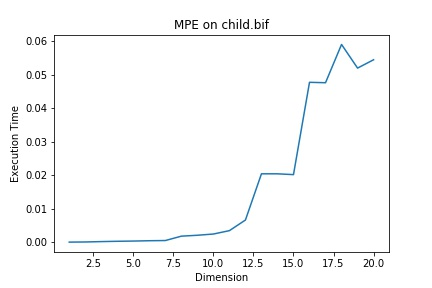
\includegraphics[width=0.9\linewidth]{dim_mpe_child}
	\label{dim_mpe_child} 
\end{minipage}

\begin{minipage}{\linewidth}
	\centering
	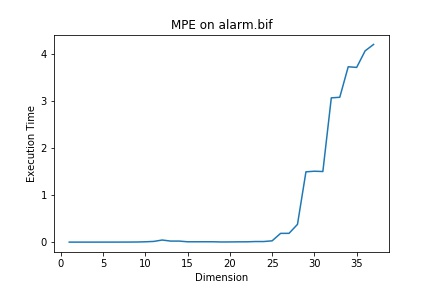
\includegraphics[width=0.9\linewidth]{dim_mpe_alarm}
	\label{dim_mpe_alarm} 
\end{minipage}
 
\begin{minipage}{\linewidth}
	\centering
	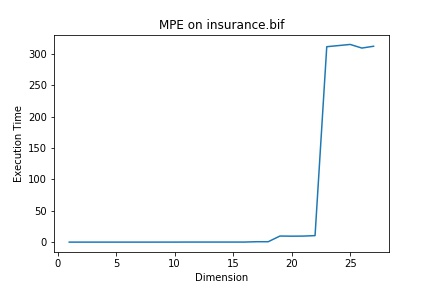
\includegraphics[width=0.9\linewidth]{dim_mpe_insurance}
	\label{dim_mpe_insurance} 
\end{minipage}

Come possiamo vedere dal grafico la complessità diminuisce mano a mano che la rete perde nodi. Come ci si potrebbe aspettare lo stesso avviene anche con il calcolo di MAP (nel caso di MAP si è scelto di selezionare di volta in volta, ed in modo casuale, un numero di variabili di MAP pari alla metà delle variabili totali rimaste). 

\begin{minipage}{\linewidth}
	\centering
	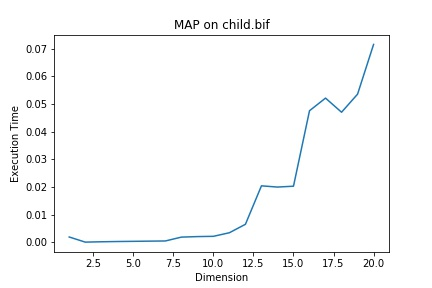
\includegraphics[width=0.9\linewidth]{dim_map_child}
	\label{dim_map_child} 
\end{minipage}

\begin{minipage}{\linewidth}
	\centering
	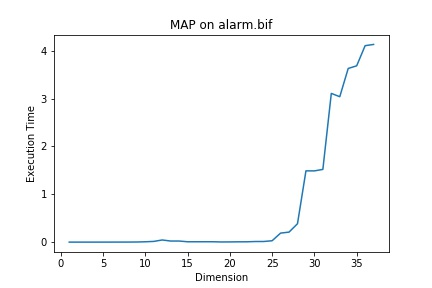
\includegraphics[width=0.9\linewidth]{dim_map_alarm}
	\label{dim_map_alarm} 
\end{minipage}
 
\begin{minipage}{\linewidth}
	\centering
	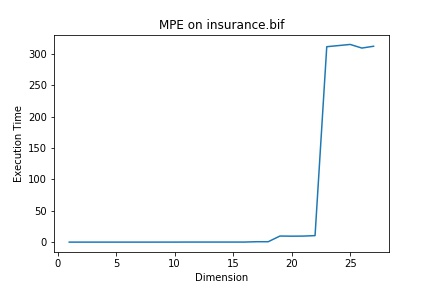
\includegraphics[width=0.9\linewidth]{dim_mpe_insurance}
	\label{dim_map_insurance} 
\end{minipage}


\section{Analisi della complessità}
Come variano le performance di MAP ed MPE al variare delle dimensioni della rete? (Dove per “complessità” si intende lontananza da un polytree). In questo caso non è stato possibile ricorrere ad un approccio completamente automatico ma ci siamo affidati ad un approccio euristico. Tra le descrizioni delle reti di esempio che ci sono state fornite vi è il campo “Average Markov Blanket Size”. Il Markov Blanket di un nodo è dato dal numero di genitori, figli e co-genitori. Questo valore indica il numero di nodi necessari affinché tale nodo risulti condizionalmente indipendente dai suoi vicini. Il valore fornito nella descrizione fornisce il livello medio generale di tutta la rete, per cui in questo contesto viene usato come stima del grado di connettività. Più questo valore è alto, più la rete è interconnessa e più è possibile trovare diversi percorsi che collegano due nodi (condizione da soddisfare per allontanarsi da un polytree). Nella scelta delle reti da usare come esempio, non è stato preso in considerazione solo il numero di nodi, ma anche questo parametro. Riprendendo i grafici appena proposti, possiamo notare che indipendentemente dal numero di nodi, il fattore di connettività maggiore sia dominante rispetto ai tempi di calcolo. Questo è reso particolarmente evidente dalla rete “Insurance” la quale, pur avendo quasi 10 nodi in meno rispetto ad alarm ha quasi due punti di AMbs in più, e infatti si può notare come i suoi tempi siano notevolmente maggiori rispetto a quelli di alarm. Da ciò se ne conclude che il numero di nodi ha un impatto sui tempi di calcolo ma questo valore dipende prevalentemente dal grado di connessione della rete (e questo vale per entrambi gli algoritmi).

\section{Analisi sul numero di variabili di evidenza}
Come variano le performance di MAP ed MPE al variare del numero di variabili di evidenza? Entrambi gli algoritmi cercano il miglior assegnamento possibile per un certo numero di variabili. Se questo numero diminuisce grazie al fatto che l’ assegnamento di alcune variabile viene già dato come input e non deve essere calcolato, è naturale pensare che l’ algoritmo necessiti di meno calcoli per arrivare alla soluzione.  L’algoritmo infatti non esegue l’ eliminazione di variabili di cui si ha già un’evidenza ed inoltre riduce tutte le cpt aventi assegnamenti incompatibili con tali evidenze (andando a ridurre notevolmente il carico di operazioni necessarie per il metodo di pointwise). Il costo complessivo è dominato dal fattore più grande che si viene a creare durante il processo, per cui limitare la grandezza della massima della cpt che si genera abbassa notevolmente i tempi di calcolo. Qui di seguito possiamo osservare dei casi di studio. 
L’andamento dei grafici conferma quanto ci si potrebbe aspettare, ovvero all’ aumentare delle evidenze il costo totale decresce.

\begin{minipage}{\linewidth}
	\centering
	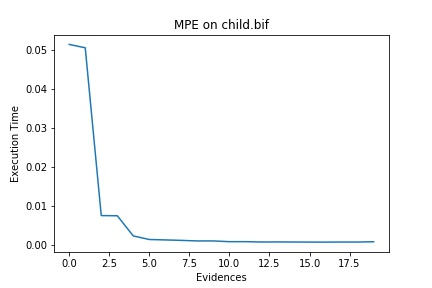
\includegraphics[width=0.9\linewidth]{evi_mpe_child}
	\label{evi_mpe_child} 
\end{minipage}

\begin{minipage}{\linewidth}
	\centering
	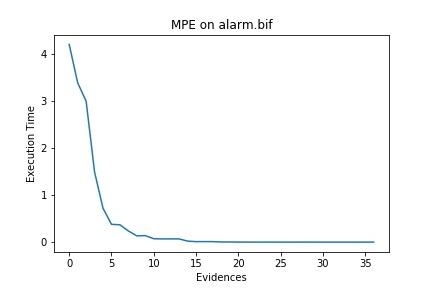
\includegraphics[width=0.9\linewidth]{evi_mpe_alarm}
	\label{evi_mpe_alarm} 
\end{minipage}
 
\begin{minipage}{\linewidth}
	\centering
	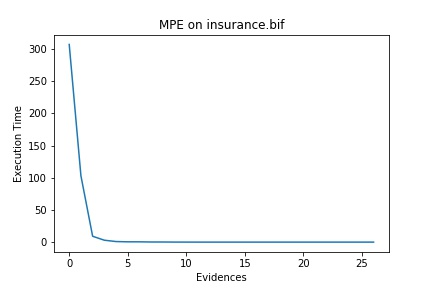
\includegraphics[width=0.9\linewidth]{evi_mpe_insurance}
	\label{evi_mpe_insurance} 
\end{minipage}

Il comportamento è lo stesso anche per MAP, in questo caso il numero di variabili di MAP selezionate corrisponde sempre alla metà di quelle totali.

\begin{minipage}{\linewidth}
	\centering
	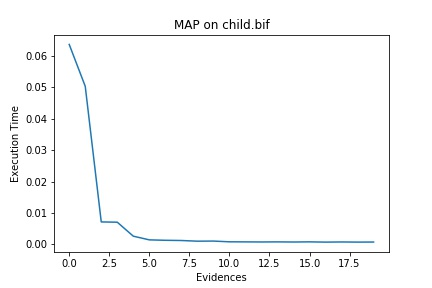
\includegraphics[width=0.9\linewidth]{evi_map_child}
	\label{evi_map_child} 
\end{minipage}

\begin{minipage}{\linewidth}
	\centering
	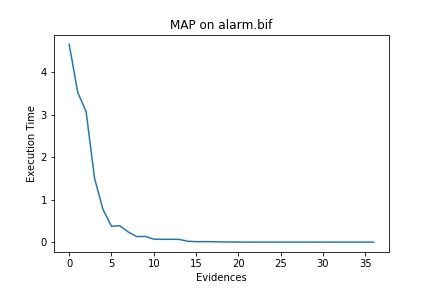
\includegraphics[width=0.9\linewidth]{evi_map_alarm}
	\label{evi_map_alarm} 
\end{minipage}
 
\begin{minipage}{\linewidth}
	\centering
	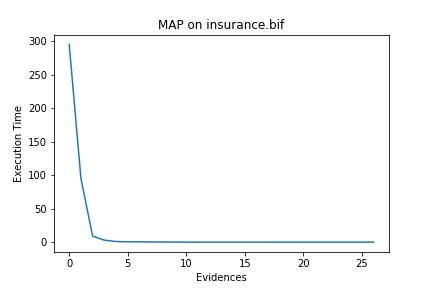
\includegraphics[width=0.9\linewidth]{evi_map_insurance}
	\label{evi_map_insurance} 
\end{minipage}


\section{Analisi sul numero di variabili di MAP}
Come variano le performance al variare del numero di variabili di MAP? Come abbiamo visto l’algoritmo di MAP esegue 2 visite della rete, la prima serve per eliminare le variabili che non sono state selezionate. Ora, dal momento che non vi sono grandi differenze tra operazioni di max out e sum out non ci si dovrebbero aspettare una crescita o decrescita lineare in base all’aumento di tali variabili. 

Lasciamo qui di seguito alcuni esperimenti effettuati su diverse reti con diverse configurazioni:

\begin{minipage}{\linewidth}
	\centering
	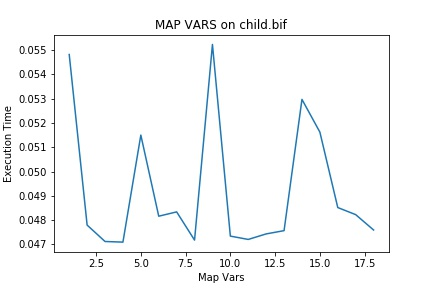
\includegraphics[width=0.9\linewidth]{map_child}
	\label{map_child} 
\end{minipage}

\begin{minipage}{\linewidth}
	\centering
	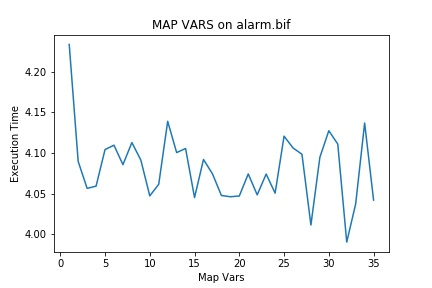
\includegraphics[width=0.9\linewidth]{map_alarm}
	\label{map_alarm} 
\end{minipage}
 
\begin{minipage}{\linewidth}
	\centering
	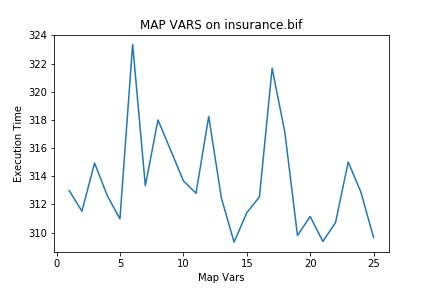
\includegraphics[width=0.9\linewidth]{map_insurance}
	\label{map_insurance} 
\end{minipage}

Ciò che si osserva è un’enorme variazione nei risultati ottenuti il che ci porta alla conclusione che le performance non sono tanto influenzate dal numero di variabili di MAP selezionate, ma dalla loro posizione all’interno della rete che influenza inevitabilmente l’ordine di eliminazione delle variabili. Infine si noti l’inefficienza di MAP rispetto al caso MPE (corrispondente alla parte finale del grafo, ovvero quella in cui vengono selezionate tutte le variabili come variabili di map). 


